


\documentclass[a4paper, 8pt, landscape]{scrartcl} %[Blattgrösse, Schriftgrösse, Orientierung]{dok. Art}
%! TEX root = ../Zsfg-PhysII-2017.tex

%Allgemein:
\usepackage[ngerman]{babel} %Neue deutsche Rechtschreibung, inkl. auto. Worttrennung (für Englisch: ngerman=english)
\usepackage[utf8]{inputenc}
\usepackage[margin=1cm]{geometry} %Blatt Ränder
\usepackage[table]{xcolor}
\usepackage{varioref}
\usepackage{booktabs} %Tabellen
%Mathematisch:
\usepackage{amsmath, parskip}
\usepackage{empheq}
\usepackage{amssymb} %für Zahlen zeichen
\allowdisplaybreaks          %erlaube Seitenumbrüche in align.
%Physikalisch:
\usepackage{siunitx} % Zahlen mit Einheiten
\usepackage{braket}
%Graphisch
\usepackage{graphicx} %Bilder einfügen
\usepackage{multicol} %Spalten
\usepackage{enumitem} %Liste



\title{Aufgabensammlung PVK NuS 1}	%Titel für \maketitel
\author{René Zurbrügg}	%Autor für \maketitel
\date{\today}		%Datum für \maketitel


\begin{document}
\begin{multicols}{2}
  \maketitle
  \begin{center}
      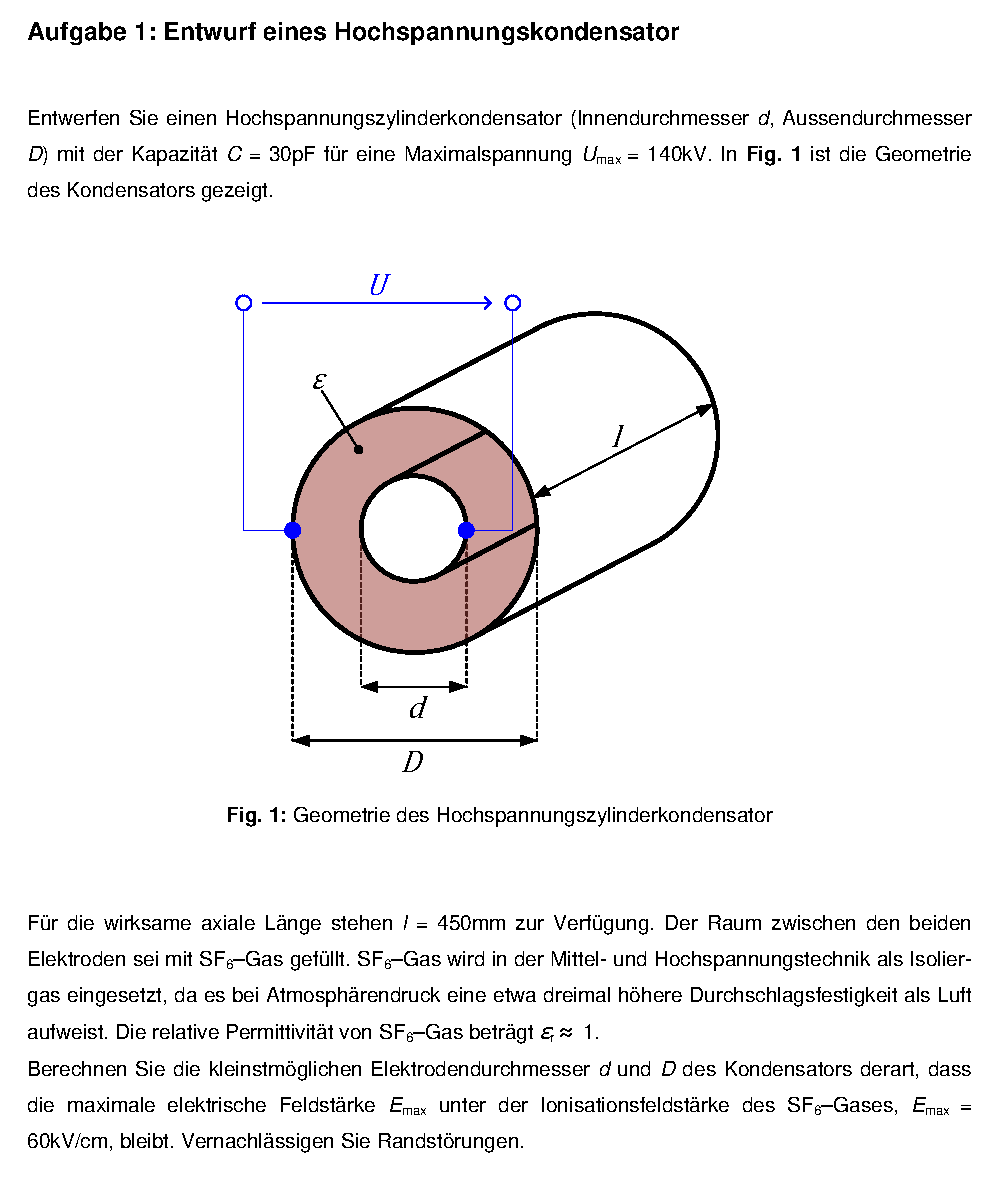
\includegraphics[width=0.8\columnwidth]{img/a1.pdf} \\
  \end{center}
    \vfill \null \columnbreak

  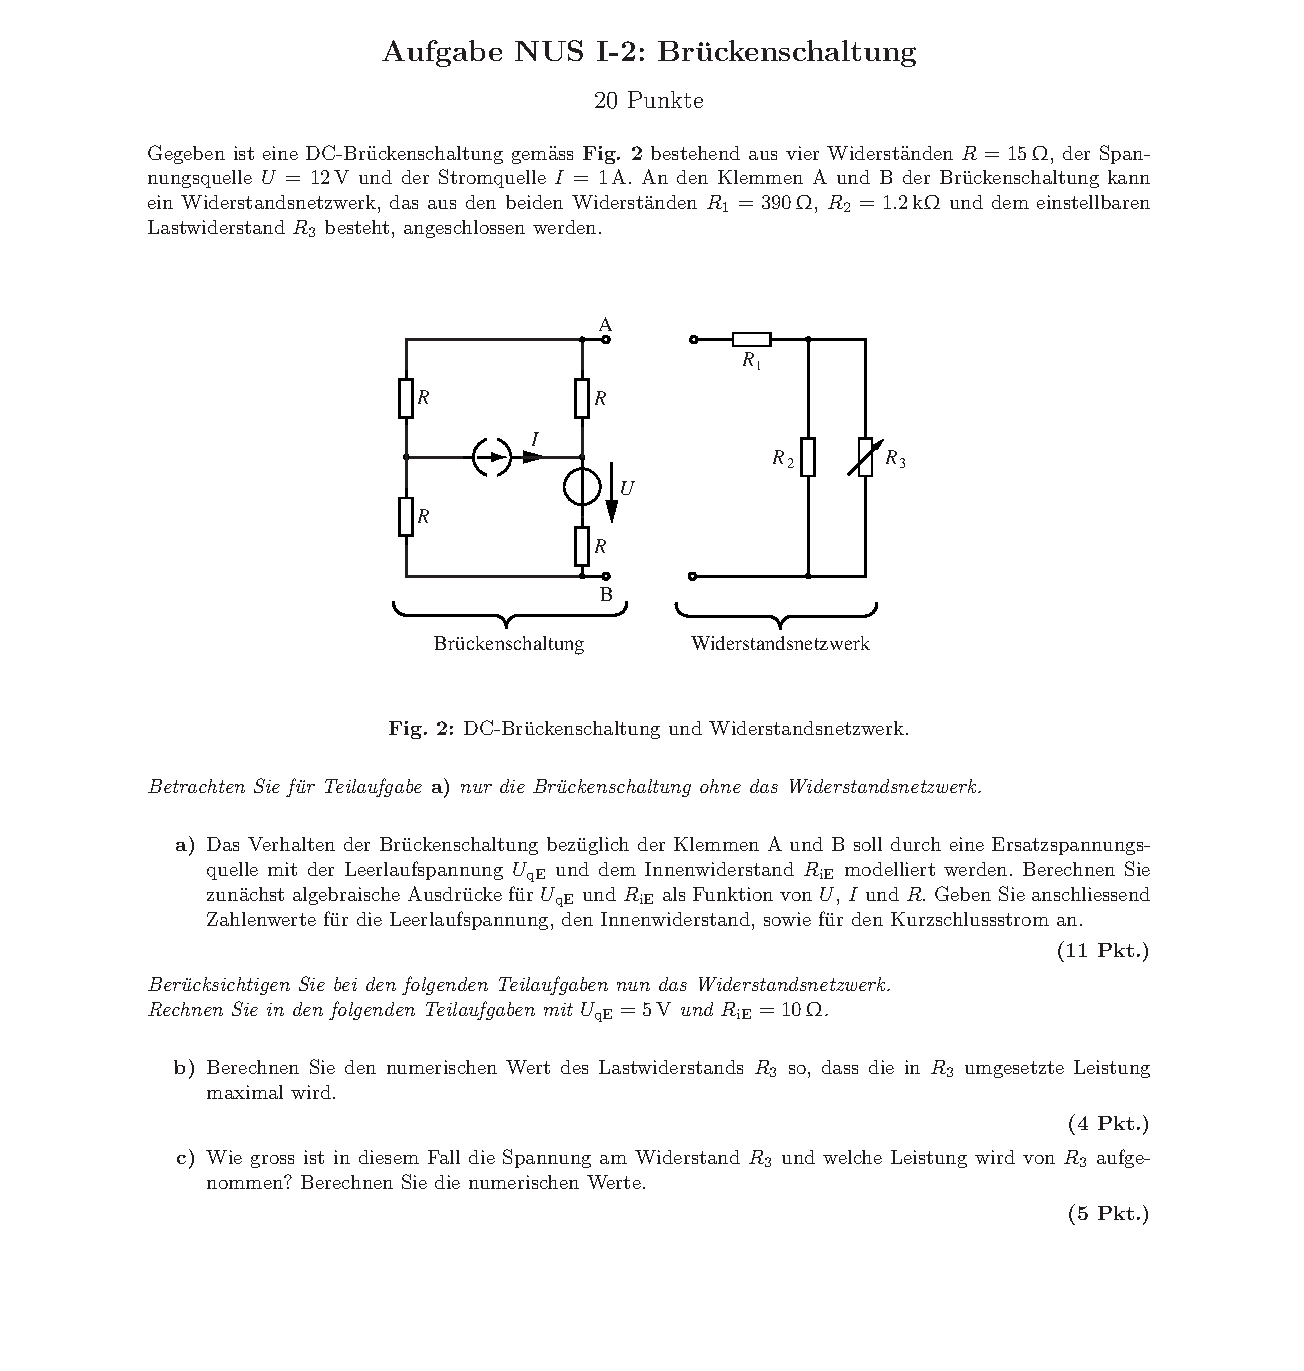
\includegraphics[width=\columnwidth]{img/a3.pdf} \\

    \vfill \null \columnbreak
    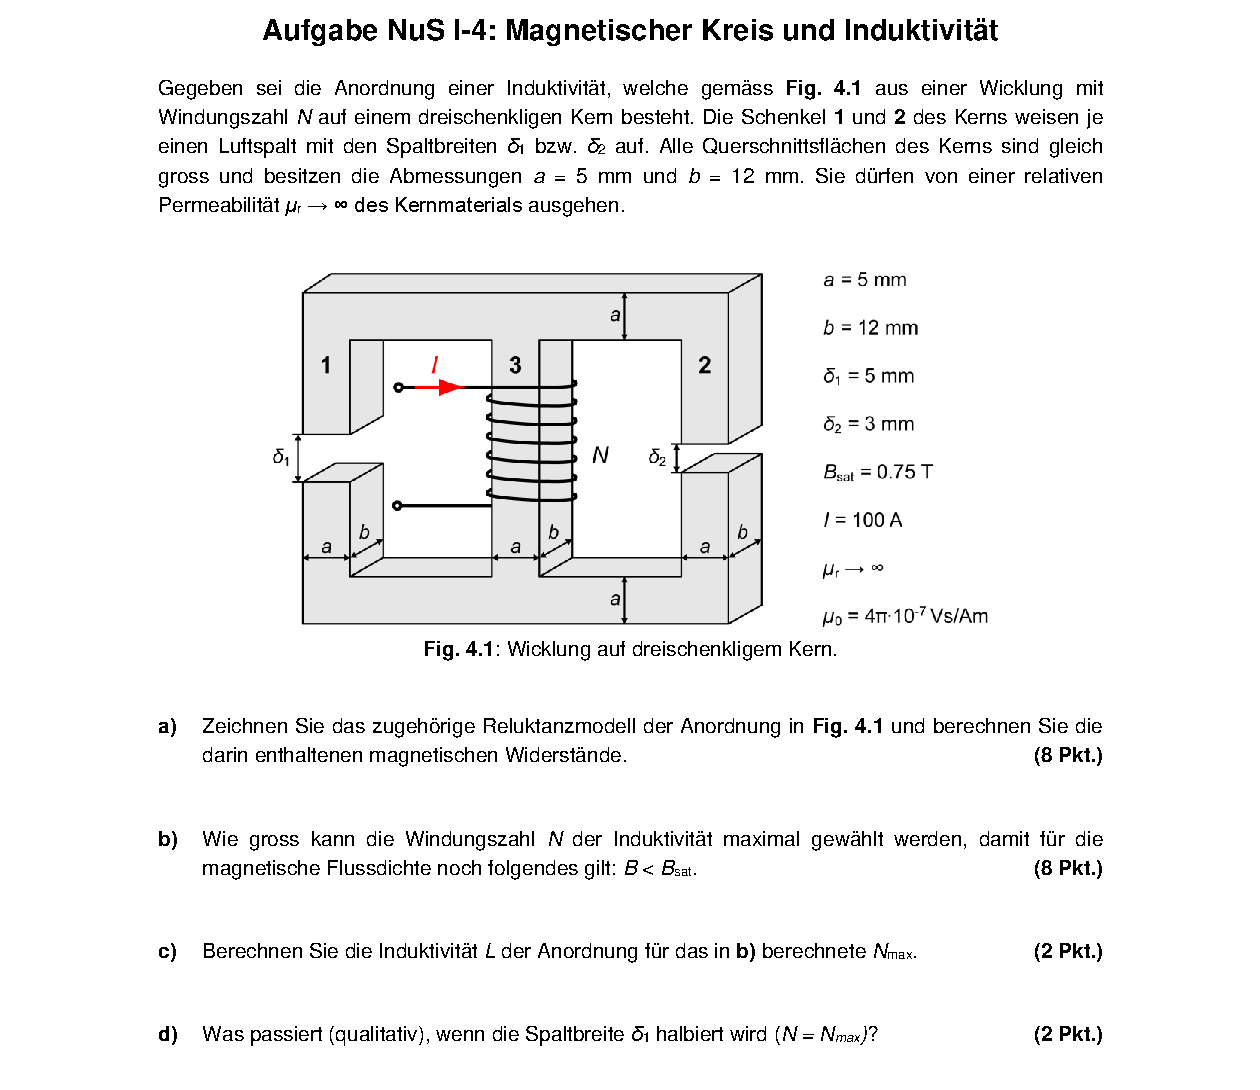
\includegraphics[width=\columnwidth]{img/a2.pdf} \\
  \vfill \null \columnbreak



  \newpage
  \section{Zusatzaufgaben}




  \begin{center}
      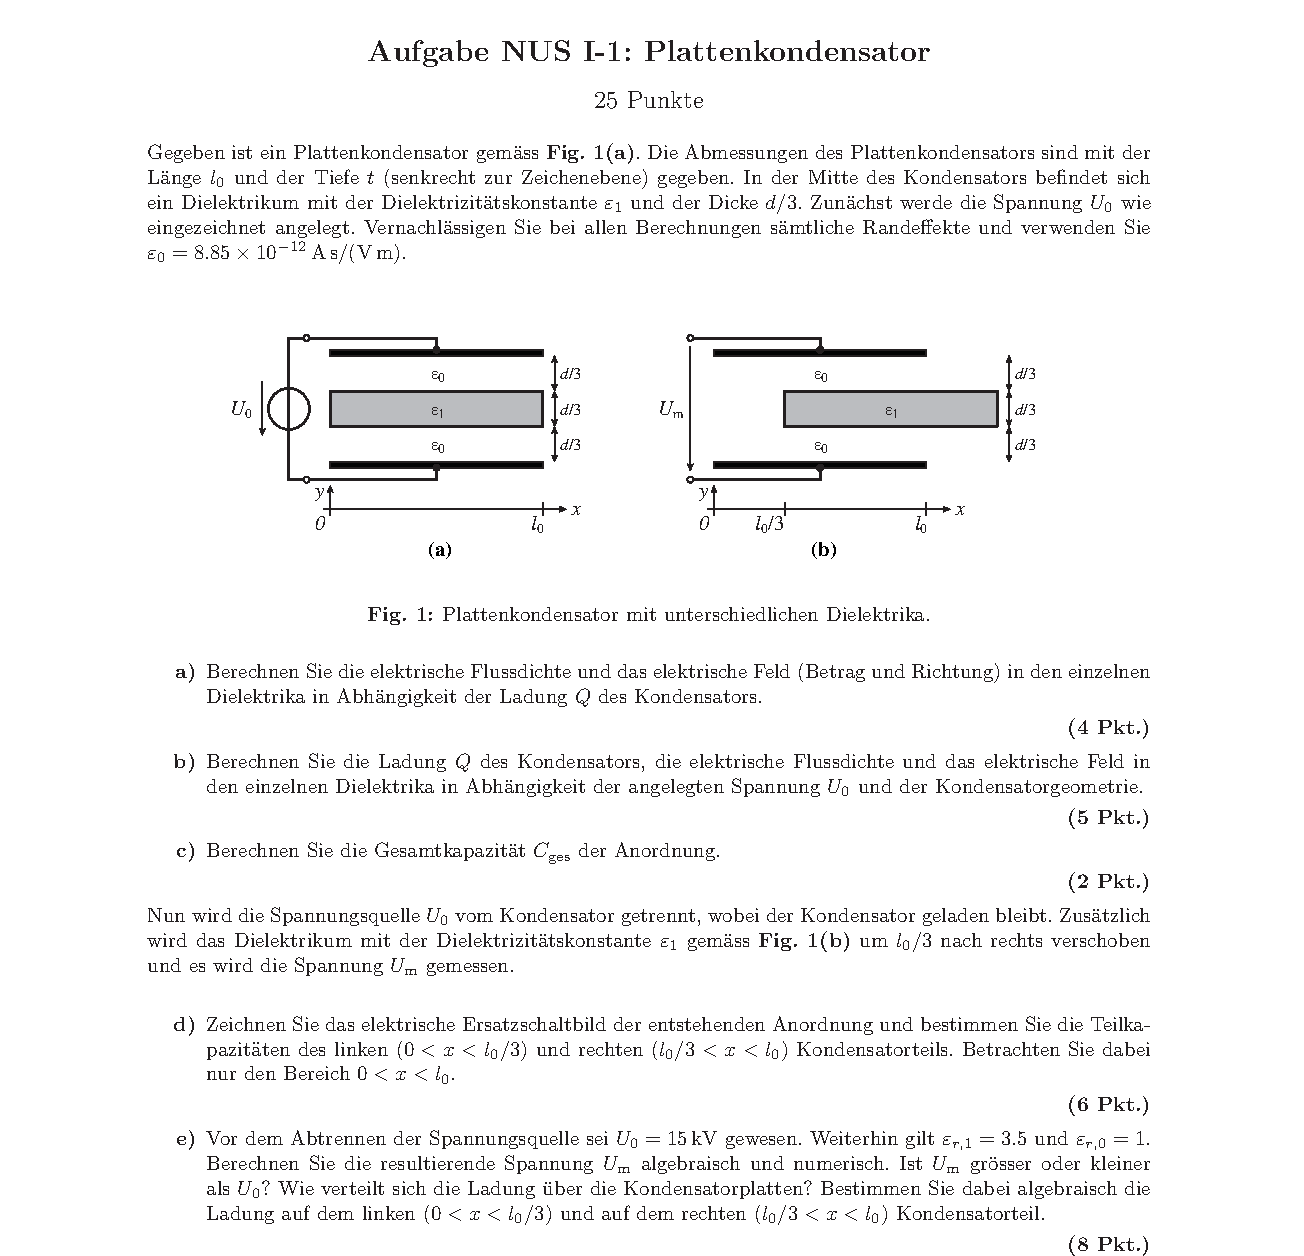
\includegraphics[width= \columnwidth]{img/efeld2.pdf} \\
  \end{center}
    \vfill \null \columnbreak

  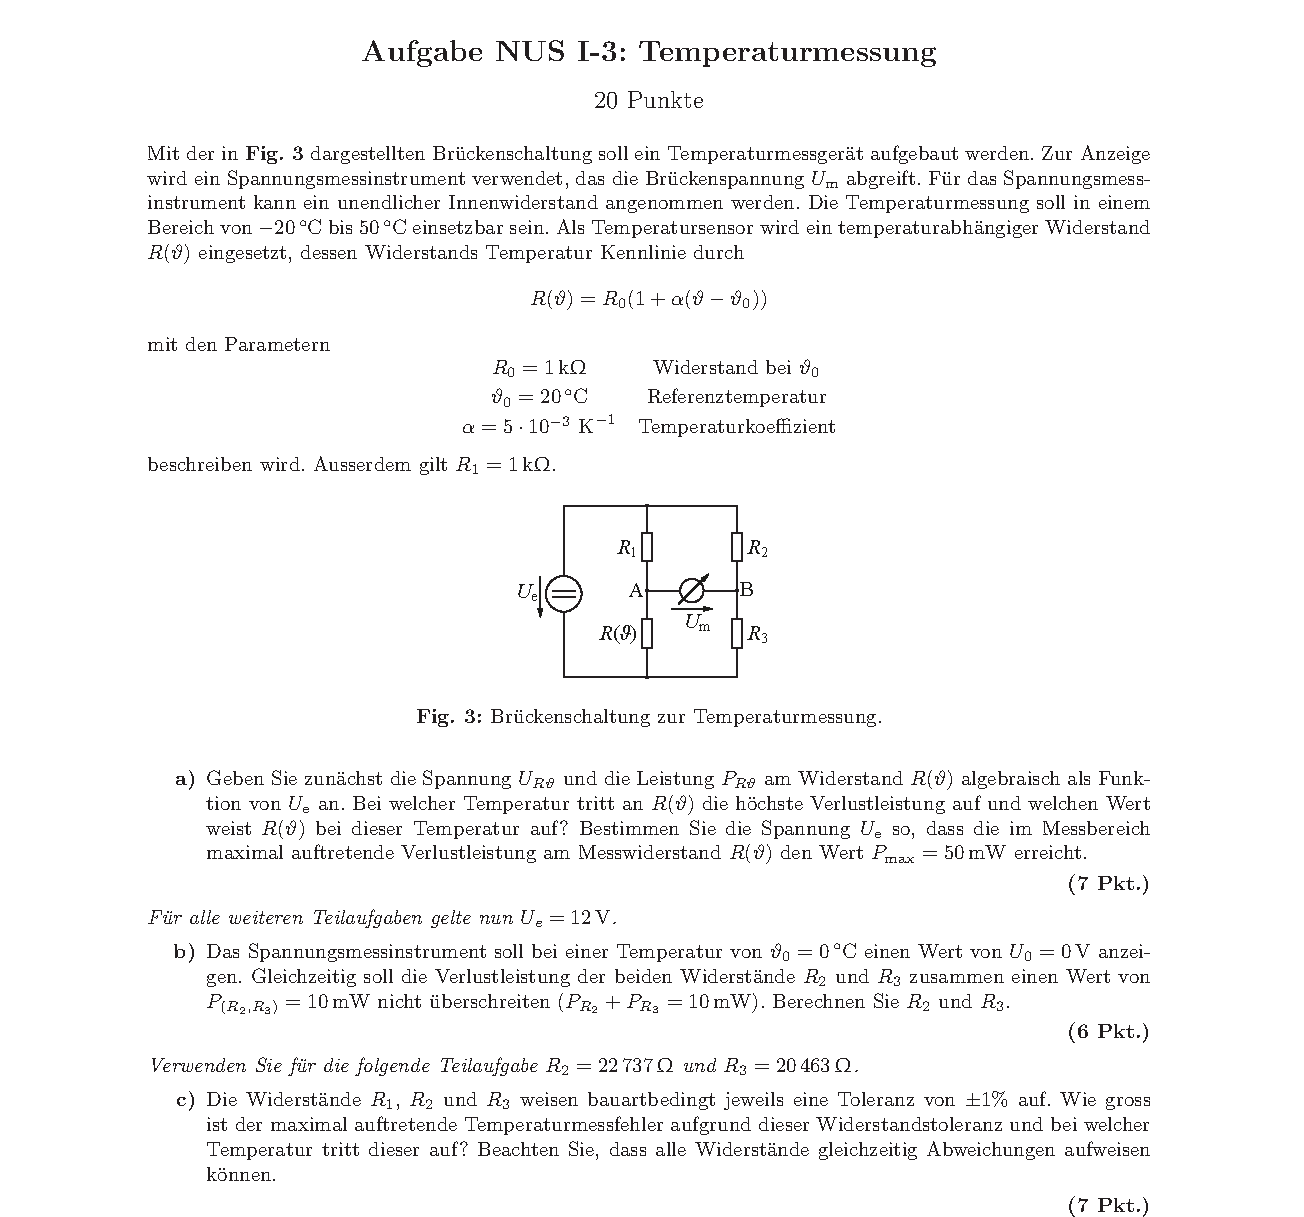
\includegraphics[width=\columnwidth]{img/netzw2.pdf} \\

    \vfill \null \columnbreak




\end{multicols}


\end{document}
